\chapter{Results}
The demonstrator can operate in two modes.
In the static mode, the trigger is deactivated and the spring is put on the glass plate with no movement.
In the dynamic mode, the demonstrator is tilted to an angle of 15 degrees, and the spring can be sided over the glass plate through the filed of view of the camera.
It is assumed that the spring moves this way with with a velocity of 2\,m/s.
It can later be shown that this velocity estimation seems accurate.

In this section we take first a look, if the software operates fast enough and how accurate the measurements are.

\section{Speed}
As stated earlier, the demonstrator is expected to deal with 200\,springs/minute which is is about 3.33\,springs/second.
The main loop itself is fast enough to deal with 15\,fps, while the trigger checks for images at a rate of 22\,fps.
In a fully synchronized system (every frame contains a spring), this would be about four times more than necessary.

But unfortunately, a problem is caused by the triggering of the image.
After the trigger detected that a spring is entering the frame, it searches in the next five frames for an image which contains the full spring an can therefore be used for measuring.
The problem is now, that the springs move with 2\,m/s to fast that in the next frame the trigger gets, the spring is already leaving the images.
This happens in about half of all measurement attempts.
But despite all this, since it works half of the time, it was possible to make the measurements at this speed nevertheless.

The question is how fast the springs are moving in the real world environment.
One spring has an approximated length of about 220\,mm.
The distance it has to cover, respectively the field of view of the camera at the given distance is about 330\,mm.
If it is assumed, that only one spring at the time is allowed in the frame and 3.33\,springs/s are expected, the velocity of the springs can be calculated as:
\begin{align*}
	v_{\text{spring}}=(0.33\,\text{m}+0.22\,\text{m})\cdot 3.33\,1/\text{s}=1.83\,\text{m/s}.
\end{align*}
2\,m/s should therefore be sufficient.

\section{Measurement accuracy}
Both the length ($L$) and the diameter ($D$) of a the steel spring, have been measured.
300 measurements were taken with no movement (static) and again 300 measurements with a moving object.
The object velocity in the horizontal direction, used for the rolling shutter correction, is estimated as 2\,m/s.
Unfortunately, the implemented trigger has it's given limitations and does not work with higher velocities.

The histograms are shown in Figure \ref{development:hist}.
The static measurements are plotted in orange and the dynamic in blue.
The label displays each mean ($\mu$) and standard deviation ($\sigma$).
\begin{figure}[ht]
	\centering
	\subfigure[\label{development:hist1}]{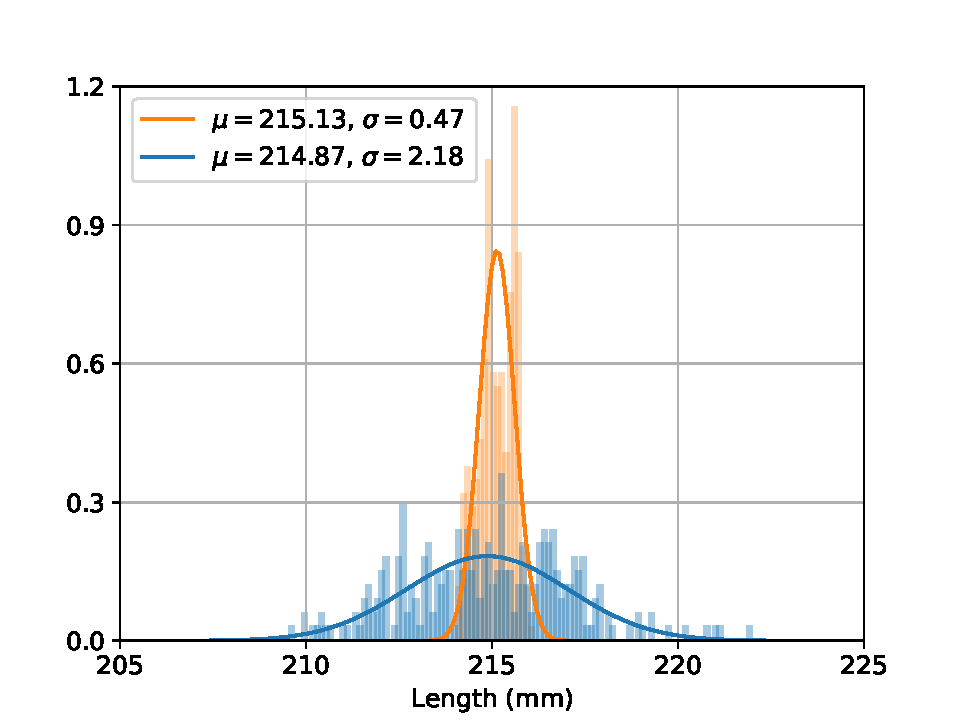
\includegraphics[width=0.45\linewidth]{4-results/images/hist_length.pdf}}
	\subfigure[\label{development:hist2}]{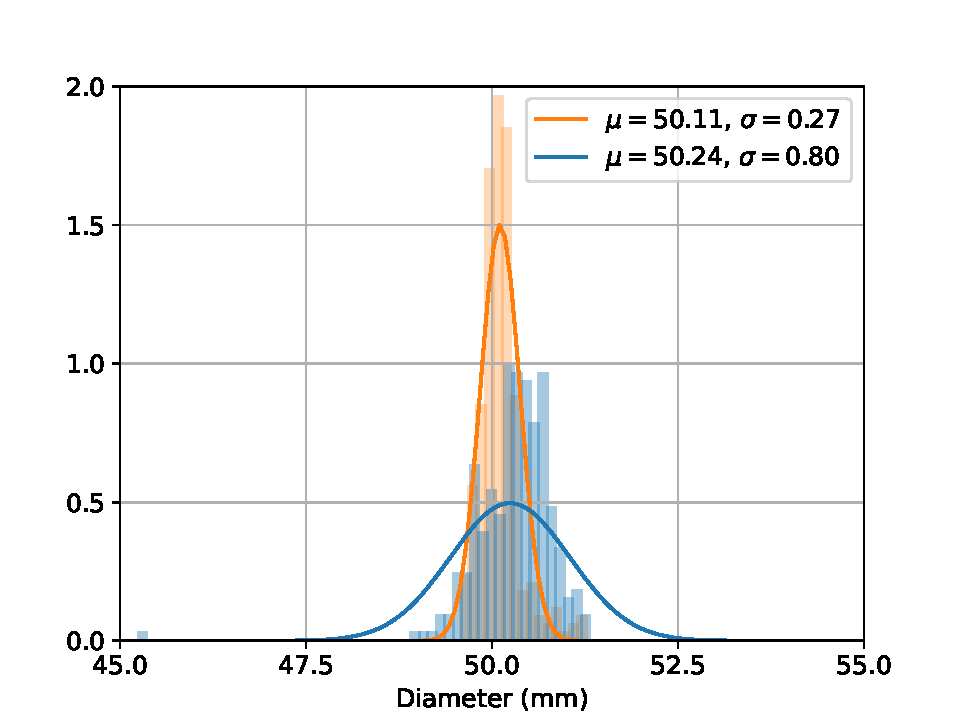
\includegraphics[width=0.45\linewidth]{4-results/images/hist_diameter.pdf}}
	\caption{Histograms of both the dynamic and static measurements\label{development:hist}}		
\end{figure}
The static and dynamic mean of the length is very similar, which indicates that the assumption that the spring moves at a speed of 2\,m/s is valid, under the condition, that rolling shutter time delay is close to the true value.

The relative errors are the computed like
\begin{align*}
	e_{L}^{\text{static}}&=\frac{0.47}{215.13}=0.22\%&e_D^{\text{static}}&=\frac{0.27}{50.11}=0.54\%\\
	e_{L}^{\text{dynamic}}&=\frac{2.18}{214.87}=1.01\%&e_D^{\text{dynamic}}&=\frac{0.8}{50.24}=1.60\%.
\end{align*}

